\documentclass[a4paper,12pt]{article}

%% Standard
\usepackage[ngerman]{babel} 
\usepackage[utf8]{inputenc}
\usepackage[T1]{fontenc}

%% Mathe
\usepackage{amsmath}
\usepackage{amssymb}
\usepackage{amsthm}
\usepackage{latexsym}

%% Aufzaehlungen
\usepackage{enumerate}

%% Bilder
\usepackage{subfigure}
\usepackage{graphicx}

%% Absaetze usw
\usepackage{multicol}   
% zu verwenden mit 
% \begin{multicols}{$$Spaltenanzahl$$} 
%  text...
% \end{multicols}

%\setlength{\parindent}{0pt}    %Absatz-Einrueckung
%\setlength{\parskip}{3pt}      %Absatz-Abstaende


%% Fusszeilen
\usepackage{fancyhdr}
\pagestyle{fancy}
\renewcommand{\headrulewidth}{0pt}
\renewcommand{\footrulewidth}{0.4pt}
\lfoot{\NAME : \TITEL}
\cfoot{}
\rfoot{\thepage}
\lhead{}
\chead{}
\rhead{}
%\setlength{\headheight}{15pt}


%% Links
\usepackage[colorlinks=true,linkcolor=black,citecolor=black,%
bookmarksnumbered=true,breaklinks=true,pdfstartview=FitH]{hyperref}

%% Eigene Kommandos
% Differenzialrechnung
\newcommand{\diff}{\ensuremath{\mathrm d}}
\newcommand{\dx}{\ensuremath{\mathrm dx}}
\newcommand{\dvx}{\ensuremath{\mathrm d \vec x}}

% Lineares
\newcommand{\Mat}[1]{\ensuremath{\mathbf{#1}}}
\newcommand{\Ten}[1]{\ensuremath{\mathcal{#1}}}
\newcommand{\Ve}[1]{\ensuremath{\vec{#1}}}
% Vektoren sind Fette buchstaben
\renewcommand{\vec}[1]{\ensuremath{\boldsymbol{#1}}}
% Vektoren sind fett und nicht kursiv
% \renewcommand{\vec}[1]{\ensuremath{\mathbf{#1}}}
\newcommand{\skp}[2]{\ensuremath{\langle #1 \,|\, #2 \, \rangle}}


% Euler
\newcommand{\e}{\ensuremath{\operatorname{e}}}
\newcommand{\E}{\ensuremath{\operatorname{e}}}
\newcommand{\ir}{\ensuremath{\operatorname{i}}}
\newcommand{\I}{\ensuremath{\operatorname{i}}}

% allg Mathe
\newcommand{\R}{\ensuremath{\mathbb{R}}}
\newcommand{\folgt}{\ensuremath{\Rightarrow}}
\newcommand{\gdw}{\ensuremath{\Leftrightarrow}}


% Formatierung
\newcommand{\abs}[0]{\bigskip\noindent}
\newcommand{\const}{\ensuremath{\text{\emph{const}}}}


% Umgebungen
\newtheorem{satz}{Satz}[section]
\newtheorem{defi}{Definition}[section]
\newtheorem{lemma}{Lemma}[section]






\begin{document}



\newcommand{\NAME}{Michael Kopp}
\newcommand{\FACH}{Grundlagenpraktikum -- Versuch E44}
\newcommand{\TITEL}{Das Problem mit der Rechtecksspannung}
\newcommand{\DATUM}{\today}


\pagestyle{plain} 
	% auskommentieren fuer fusszeile



%%%% Eigener Kopf

\sloppy

\begin{center}
\FACH
\hfill
\DATUM
\end{center}

\vspace{-5mm} % weniger abstand

\begin{center}
  \begin{Large}
 \textbf{\TITEL}
  \end{Large}
\end{center}

\vspace{-3mm}

\begin{center}
\hrulefill
%\quad
 %\raisebox{-1.5mm}{\NAME}
% \,
\quad 
\textit{\NAME}
\,
\hrulefill
\end{center}
 
 
%%%%%%%%%%%%%%%%%%%%%%%%%%%%%
%%%%%%%%%%%%%%%%%%%%%%%%%%%%%%
%%%%%%%%%%%%%%%%%%%%%%%%%%%%%%%%

\noindent
Ich gehe davon aus, dass der Leser mit dem Versuch E44 -- also
insbesondere dem Aufbau und der Durchf"uhrung -- vertraut ist.

\abs
Aus dem Induktionsgesetzt folgt, dass die Induktionsspannung in der
kleinen Spule proportional zur "Anderung des $B$-Feldes ist:
\begin{equation}
  \label{eq:1}
  U_i = - n \dot \Phi = - n \dot B A \;,
\end{equation}
(mit $n$: Windungszahl der kleinen Spule, $A$: Fl"ache der gro"se
Spule) wobei wiederum die "Anderung von $B$ mit der "Anderung des Stroms $I$ in
der gro"sen Spule einhergeht; f"ur die Spaltmitte gilt n"amlich
\begin{equation}
  \label{eq:2}
  B = \mu \frac{ N I }{l}
\end{equation}
($N$: Windungszahl der gro"sen Spule, $l$: L"ange der gro"sen Spule).

Um nun den Strom $I$ zu bestimmen, verwendet man das Ohmsche Gesetz $I
= U / R$ am Ohmschen Widerstand mit $R = 1 \Omega$. Die Spannung, die
hier gemessen wird, ist $U_a$, also gilt
\begin{equation}
  \label{eq:3}
  I = \frac{U_a}{R} \;.
\end{equation}
Um diese Spannung $U_a$ nun bestimmen zu k"onnen, greift man auf die
"Ubertragungsfunktion $(U_a / U_e) = :q(\omega)$ zur"uck, die in dem
Versuch mit hinreichender Genauigkeit best"atigt wurde. Damit schreibt
man n"amlich statt \eqref{eq:3}
\begin{equation}
  \label{eq:4}
  I = q(\omega) \cdot \frac{U_e}{R} \;,
\end{equation}
wobei man die Spannung $U_e$ genau kennt: Schlie"slich ist es die
eingegebenen Sinus-/Dreiecks-/Rechtecksspannung, die man zudem auf dem
Oszilloskop "uberwachen kann.

Setzt man nun  \eqref{eq:4} in \eqref{eq:2} ein und leitet nach der
Zeit ab, so kann man den Ausdruck \eqref{eq:1} wie folgt schreiben:
\begin{equation}
  \label{eq:5}
  U_i = - n A \mu \frac{N}{l} \frac{1}{R} \, q(\omega) \, \dot U_e =:
  \kappa \, q(\omega) \, \dot U_e \;.
\end{equation}

Was man nun aber nicht beachtet hat, ist, dass \eqref{eq:5} in Strenge
nur f"ur Sinusspannungen gilt -- bspw. verwendet man bei der
Herleitung von $q(\omega)$ den (komplexen) Widerstand einer Spule zu $Z_L = \I
\omega L$. Die Herleitung diese Terms erfolgt unter der expliziten
Annahme, dass Strom und Spannung von der Gestalt 
\begin{equation}
  \label{eq:6}
\psi(t) = \hat \psi \,\exp( \I \omega t + \varphi)  \text{ oder }
\psi(t) = \hat \psi \, \cos( \omega t + \varphi )
\end{equation}
sind.

\abs
Da wir nun aber kein Sinusf"ormiges, sondern bspw. ein Kastenf"ormiges
Potential f"ur $U_e$ verwenden, m"ussen wir dieses in Terme der
Gestalt \eqref{eq:6} entwickeln -- also eine
\emph{Fouriertransformation} durchf"uhren.

Die Rechtecksfunktion 
\begin{equation*}
  f(x) =
  \begin{cases}
    2 & 0 < x < \pi \\
    -2 & -\pi < x < 0 \\
    0 & \text{sonst}
  \end{cases}
\end{equation*}
wurde Fourierzerlegt. Aus Symmetriegr"unden fallen alle Cosinusterme
weg und f"ur die Sinusterme gilt
\begin{equation*}
  a_n = \frac{4}{\pi \, n} ( 1 - (-1)^n ) \;;
\end{equation*}
sodass die Funktion $f$ -- die unere Spannung $U_e$ sein soll -- geschrieben werden kann als Grenzwert 
\begin{equation}
  \label{eq:7}
  U_e(t) = \sum_{\omega \in \mathbb Z^\ast} \frac{4}{\pi \, \omega} ( 1 -
  (-1)^\omega ) \, \sin( \omega t) \;.
\end{equation}
Nach Fej\'er konvergiert die Cesarosumme dieser Reihe gleichm"a"sig,
desweiteren sind die einzelnen Glieder beschr"ankt; damit darf man
Reihe und Ableitung vertauschen sofern die folgende Reihe
existiert.... Man erh"alt dann
\begin{equation}
  \label{eq:8}
  \dot U_e = \sum_{\omega \in \mathbb Z^\ast} \frac{4}{\pi} ( 1 -
  (-1)^\omega ) \, \cos( \omega t) \;;
\end{equation}
vergleiche Abb. \ref{fig:delta} \;.


\begin{figure}
  \centering
  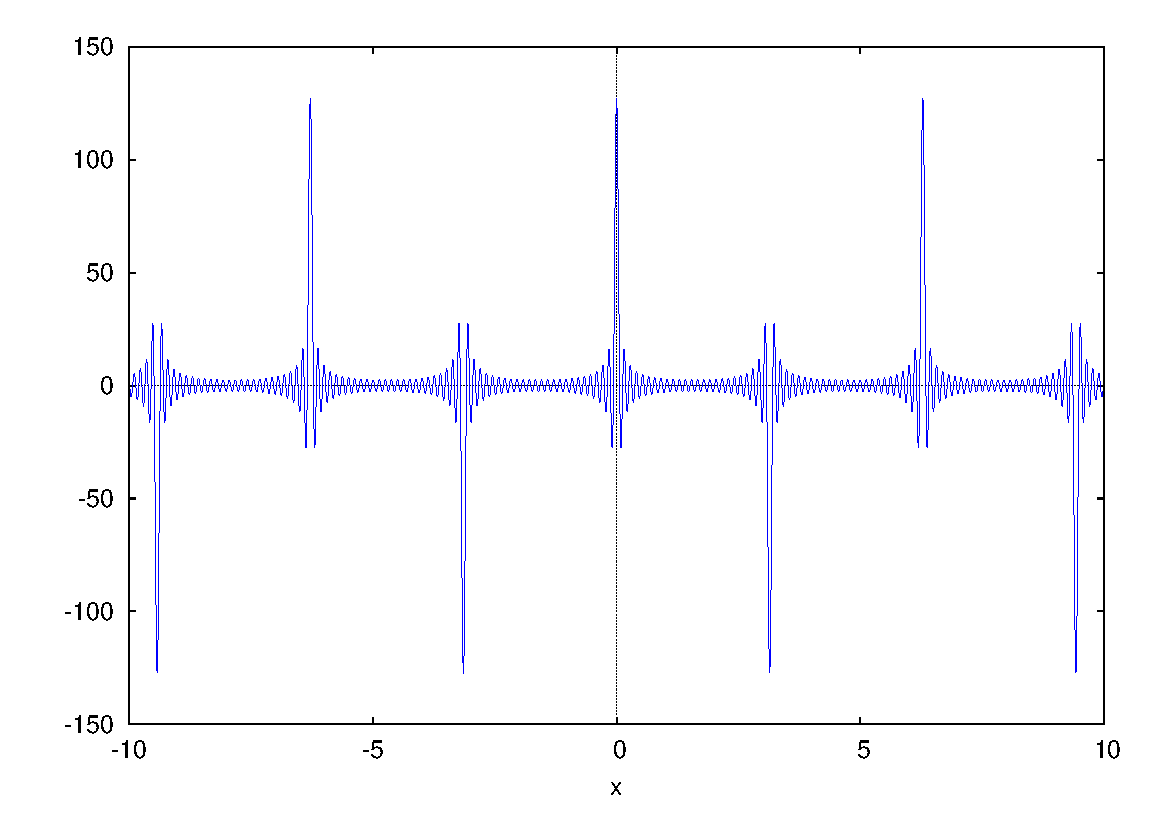
\includegraphics[width=0.8\textwidth]{delta}
  \caption{Abbildung der Funktion aus Gl \eqref{eq:8} -- dies ist die
    Partialsumme mit $\omega$-Termen aus $\{ -50, 50 \}$.}
  \label{fig:delta}
\end{figure}


Hier wurde aber noch nicht die "Ubertragungscharacteristik $q(\omega)$
einbezogen. Sie ist gegeben durch
\begin{equation}
  \label{eq:9}
  q(\omega) = \frac{R}{\sqrt{ \omega^2 L^2 + (R + R_S)^2} }
\end{equation}
und muss jetzt f"ur jeden Term in \eqref{eq:8} angewandt werden:
\begin{equation}
  \label{eq:10}
  \dot U_e = \sum_{\omega \in \mathbb Z^\ast} \frac{R}{\sqrt{ \omega^2
      L^2 + (R + R_S)^2} } \, \frac{4}{\pi} ( 1 -
  (-1)^\omega ) \, \cos( \omega t) \;.
\end{equation}
Als Zahlenwerte w"ahle ich $R = 1$,
$R+R_S = 1.4$ und $L = 0.000137$, was sich aus den experimentellen
Werten ergibt.

Betrachtet man Abb.

so sieht man, dass die Korrekturen sehr wohl zu eienr Deformation der
Kurvew f"uhren -- aber dass sie grob die selbe ist: Der Kurvenverlauf
sieht weiterhin wie der einer Deltafunktion aus.

\begin{figure}
  \centering
  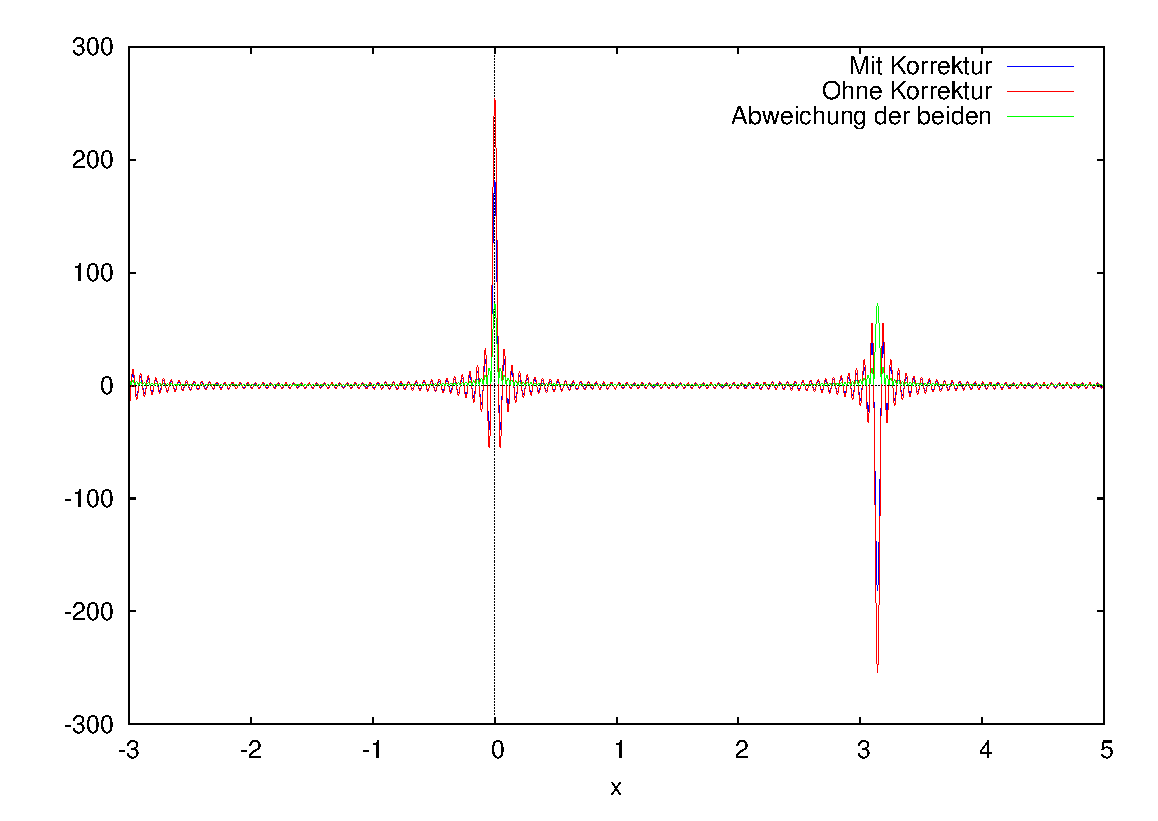
\includegraphics[width=0.8\textwidth]{vgl1}
  \caption{Vergleich der Reihen aus \eqref{eq:10} und \eqref{eq:8}
    sowie deren absolute Abweichung; bis zu Termen mit $\omega = 100$
  summiert.}
  \label{fig:vgl1}
\end{figure}

\begin{figure}
  \centering
  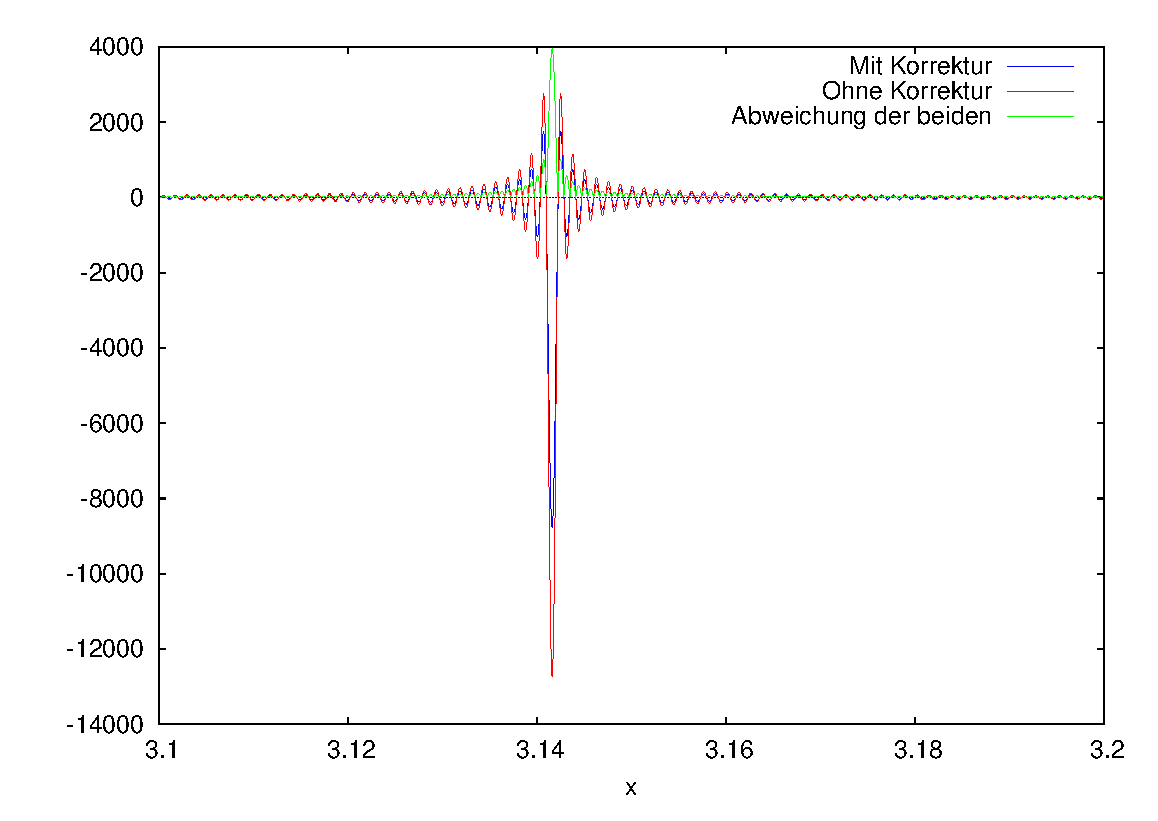
\includegraphics[width=0.8\textwidth]{vgl2}
  \caption{Vergleich der Reihen aus \eqref{eq:10} und \eqref{eq:8}
    sowie deren absolute Abweichung; bis zu Termen mit $\omega = 5000$
  summiert.}
  \label{fig:vgl2}
\end{figure}



Das war halb zu erwarten, weil die "Ubertragungsfunktion \eqref{eq:9}
f"ur kleine Werte $\omega$ recht konstant ist; vgl Abb. \ref{fig:uebertr}
und beachte die Skalierung. Die Komponenten der Reihe \eqref{eq:10}
mit hohem $\omega$ st"oren den Gruns"atzlichen Verlauf der Kurve immer
weniger, weil die h"oheren Frequenzen nur noch schmale "`Zacken"'
einbringen... Werden sie von $q$ abgeschnitten, so sorgen sie damit
nur noch f"ur eine fehlende Verschm"alerung der $\delta$-Funktion.

\begin{figure}
  \centering
  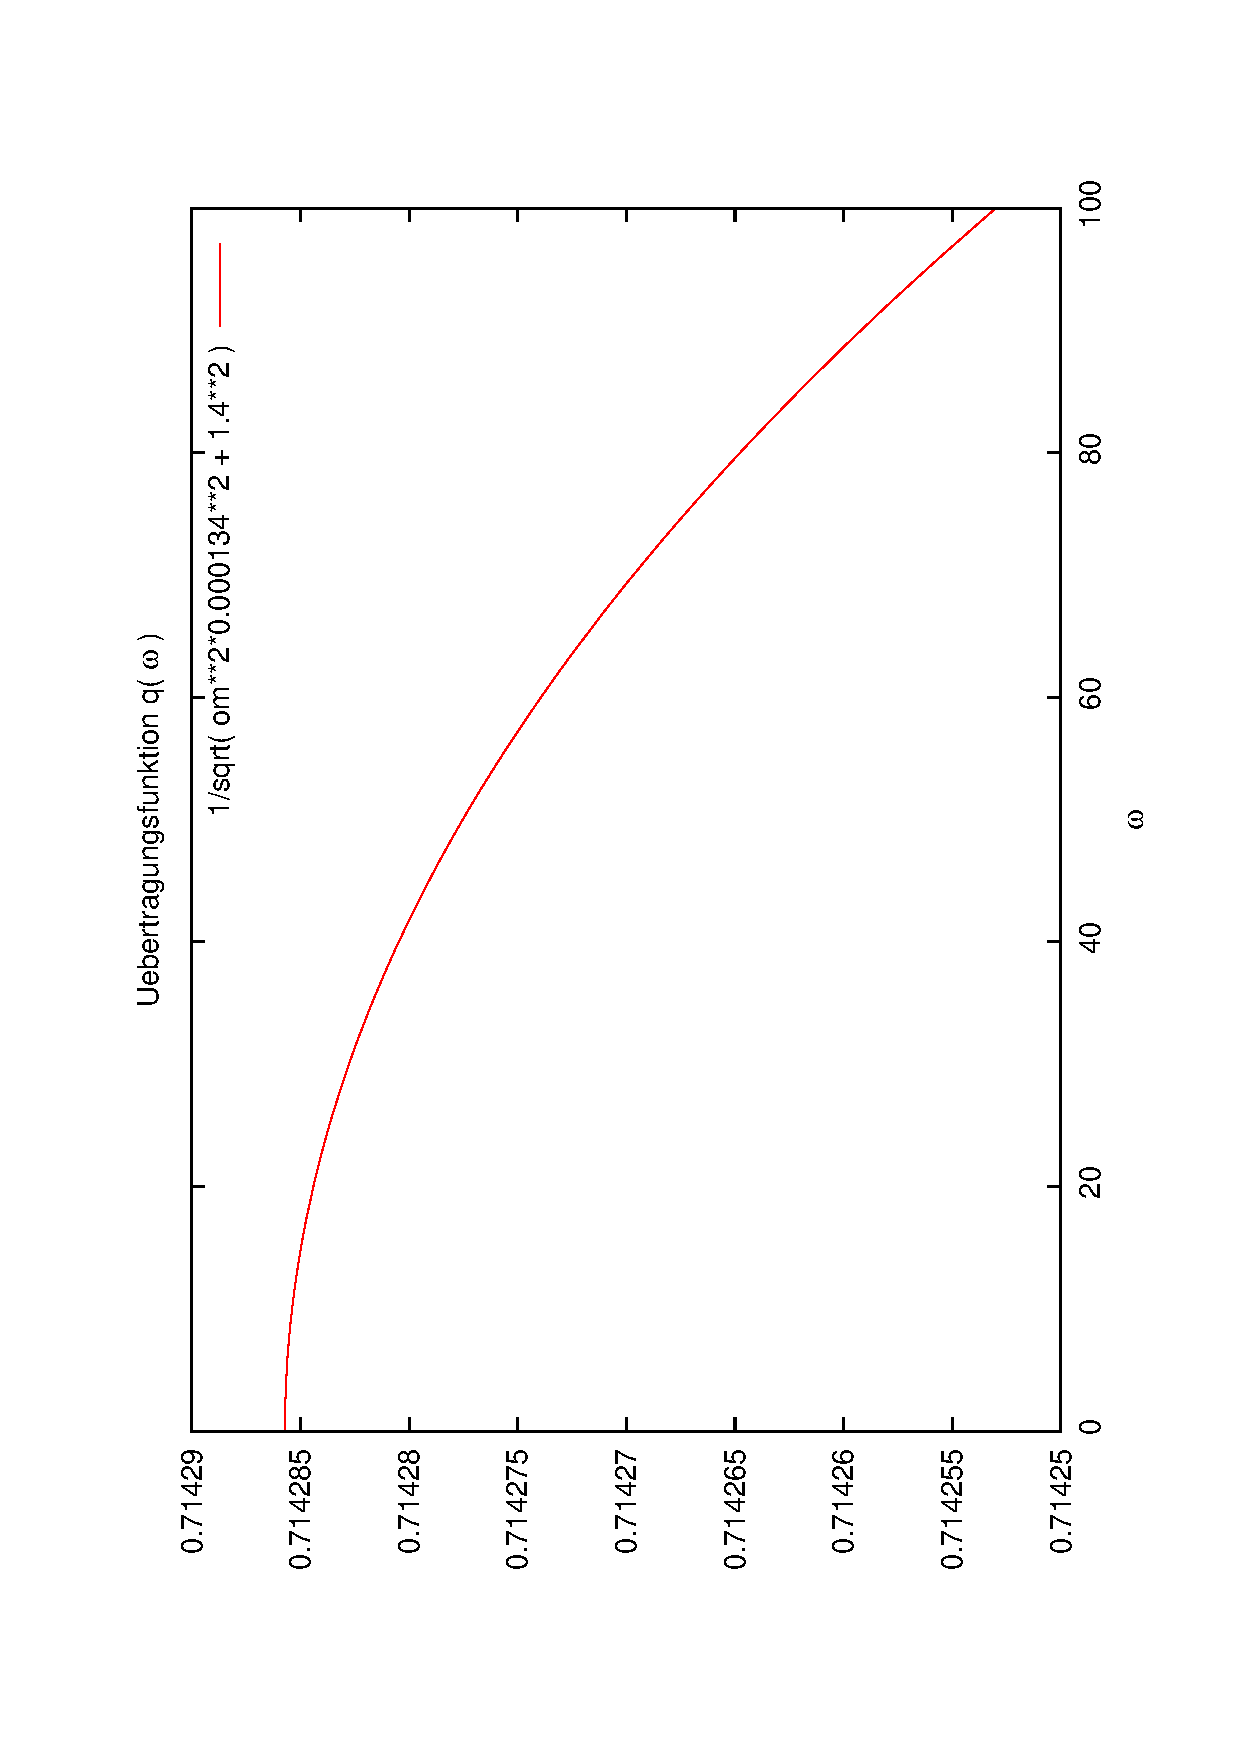
\includegraphics[width=0.8\textwidth,height=0.4\textheight]{uebertr}
  \caption{"Ubertragungsfunktion $q(\omega)$ f"ur "`kleine"' Frequenzen $\omega$}
  \label{fig:uebertr}
\end{figure}
 


\abs
Nach diesen Ergebnissen kann man das $q$ in \eqref{eq:5} getrost
konstant setzen und sich an dem Zusammenhang
\begin{equation}
  \label{eq:11}
  U_i \propto \dot U_e 
\end{equation}
erfreuen.

Andere Einflu"usse, die \eqref{eq:11} nichtig machen, m"ochte ich
hiermit aber keinesfalls ausschlie"sen, sondern nur \emph{eine}
Fehlerquelle relativieren...


\abs
Um die Rechnungen nachvollziehen zu k"onnen hier die
\texttt{Maxima}-Funktionen, mit denen ich gerechnet habe. Weil mein PC
nicht der schnellstes ist, konnte ich nicht mit beliebig hohen
$\omega$ arbeiten...

\begin{verbatim}
S(k) := sum( 4/%pi * (1-(-1)**n) * cos(n*x), n, -k, k );
q(n) := 1/sqrt( n**2 * 0.000137**2 + 1.4**2 );
T(k) := sum( q(n) * 4/%pi * (1-(-1)**n) * cos(n*x), n, -k, k );
plot2d( [T(100), S(100), abs(T(100) - S(100)) ], [x,-3,5] , 
    [legend, "Mit Korrektur", "Ohne Korrektur", "Abweichung der beiden"] 
);
\end{verbatim}
 
 
 
 
 
 



\end{document}














%%% Local Variables: 
%%% mode: latex
%%% TeX-master: t
%%% End: 
